\begin{flushleft}

\chapter{Materials and Methods}

\section{Disclosure}
Parts of this chapter have been adopted in a joint first-author publication \textit{The drug-induced phenotypic landscape of colorectal cancer organoids} \parencite{betgeDruginducedPhenotypicLandscape2022}.  

\section{Patients}
All patients were identified at the University Hospital Mannheim, Mannheim, Germany. Untreated patients with a new diagnosis of colorectal cancer were included in this study. Biopsies were obtained from their primary tumors and adjacent normal tissue via forceps-based endoscopy. Exclusion criteria were active HIV, HBV or HCV infections. Biopsies were transported in phosphate buffered saline (PBS) on ice. Clinical data, tumor characteristics and molecular tumor data were pseudonymized. The study was approved by the Medical Ethics Committee II of the Medical Faculty Mannheim, Heidelberg University (Reference no. 2014-633N-MA and 2016-607N-MA). All patients gave written informed consent before tumor biopsy was performed. The initial cohort consisted of organoids from 25 patients with colorectal cancer, 10 of them female, 15 male, with a mean age of 66 years.

\begin{table}[htbp]
\caption{Patient derived organoid Lines}
\label{tab:patient_organoid}
\begin{tabularx}{\textwidth}{lXXXXX}
\toprule
\textbf{Line} & \textbf{Optimal medium} & \textbf{Qualitative growth} & \textbf{Patient sex} & \textbf{Location} & \textbf{UICC stage} \\
\midrule
D004T & ENA & good & female & rectum & 3 \\
D007T & ENA & good & m & rectum & 3 \\
D010T & ENA & good & female & sigmoid & 3 \\
D013T & ENAS & good & m & rectum & 1 \\
D015T & ENA & good & m & descending & 2 \\
D018T & ENA & good & female & sigm & 1 \\
D019T & ENA & good & m & sigmoid & 2 \\
D020T & ENA & good & m & rectum & 1 \\
D021T & ENA & medium & m & rectum & 1 \\
D022T & ENA & good & m & ascending & 4 \\
D027T & ENA & good & female & rectum & 2 \\
D030T & ENA & good & female & ascending & 2 \\
D046T & ENA & good & female & rectum & 3 \\
\bottomrule
\end{tabularx}
\end{table}


\section{Organoid Culture}

\subsection{Patient Derived Organoid Culture}
Patient derived organiod (PDO) cultures were extracted from biopsies as reported by Sato et al. \parencite{satoLongtermExpansionEpithelial2011} with slight modifications. Tissue fragments were washed in DPBS (Life technologies) and digested with Liberase TH (Roche) before embedding into BME R1 (Trevigen). The medium, termed ENA, contained Advanced DMEM/F12 (Life technologies) medium with 1\% v/v penicillin/streptomycin (Life Technologies), Glutamax and HEPES (basal medium) supplemented with 100 ng/ml Noggin (Peprotech), B27 (Life technologies), 1,25 mM n-Acetyl Cysteine (Sigma), 10 mM Nicotinamide (Sigma), 50 ng/ml human EGF (Peprotech), 10 nM Gastrin (Peprotech), 500 nM A83-01 (Biocat), 10 nM Prostaglandin E2 (Santa Cruz Biotechnology), 10 μM Y-27632 (Selleck chemicals) and 100 mg/ml Primocin (Invivogen). After isolation, cells were kept in 2 conditions including medium as described (ENA), or supplemented with additional 3 uM SB202190 (Biomol) (ENAS) as described by Fujii et al. \parencite{Fujii2016-ax}. 
The tumor niche was determined after 14 days and organoids were subsequently cultured in the condition with best growth. 
Organoids were passaged every 7 days and medium was changed every 2-3 days.

\begin{table}[htbp]
\caption{Basal Medium Components}
\label{tab:basal_medium_components}
\begin{tabularx}{\textwidth}{Xll}
\toprule
\textbf{Component} &  \textbf{Concentration} & \textbf{Manufacturer} \\
\midrule
Advanced DMEM/F12 & 97\% v/v & Life technologies; Carlsbad, California, USA \\
GlutaMAX™ (100x) & 1\% v/v & Life technologies; Carlsbad, California, USA \\
Pen/Strep (100x) & 1\% v/v & Life technologies; Carlsbad, California, USA \\
1 M HEPES (100x) & 1\% v/v & Sigma-Aldrich Life Science/Merck, St. Louis, Missouri, USA \\
\bottomrule
\end{tabularx}
\end{table}

\begin{table}[htbp]
\caption{ENA Medium Components}
\label{tab:ena_medium_supplements}
\begin{tabularx}{\textwidth}{Xll}
\toprule
\textbf{Supplement} & \textbf{Concentration} & \textbf{Manufacturer} \\
\midrule
Basal Medium (described above) & 98\% v/v & Produced In-House \\
B27 (50x) & 2\% v/v & Life technologies; Carlsbad, California, USA \\
N-Acetylcysteine & 1.25 mM & Sigma/Merck; St. Louis, Missouri, USA \\
Human EGF & 50 ng/ml & PeproTech; Hamburg, Germany \\
Noggin & 100 ng/ml & PeproTech; Hamburg, Germany \\
Y-27632 & 10 µM & Selleck chemicals; Houston, Texas, USA \\
A83-01 & 500 nM & BioCat; Heidelberg, Germany \\
Prostaglandin E2 & 10 nM & Santa Cruz Biotechnology \\
Gastrin & 10 nM & PeproTech; Hamburg, Germany \\
Nicotinamide (Vit. B3) & 10 mM & Sigma/Merck; St. Louis, Missouri, USA \\
Primocin & 100 µg/ml & Invivogen; San Diego, California, USA \\
\bottomrule
\end{tabularx}
\end{table}


\begin{figure}[!h]
\centering
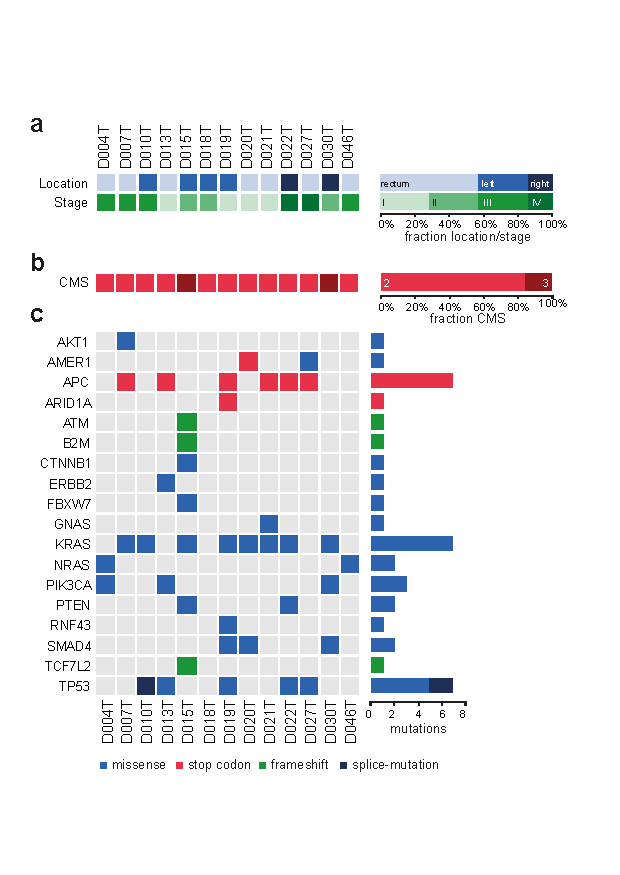
\includegraphics[width=250pt,
                height=\textheight,
                keepaspectratio]{figures/promise/pdf/fig_1_0.pdf}
\caption[Patient derived organoid cohort overview]{\textbf{Patient derived organoid cohort overview a} Tumor location (right/left/rectum) and AJCC/UICC stage of colorectal cancers that patient derived organoids were derived from. \textbf{b}  Consensus molecular subtypes of organoids determined by RNA expression analysis. \textbf{c} Mutation status in patient derived organiods, as analyzed by amplicon sequencing. Figure created with support from Johannes Betge (graphical presentation),  Erica Valentini (sequencing data analysis) and Benedikt Rauscher (CMS type inference). Figure adapted from \textit{The drug-induced phenotypic landscape of colorectal cancer organoids} \parencite{betgeDruginducedPhenotypicLandscape2022}}
\label{fig_120}
\end{figure}


\subsection{Mouse Organoid Culture}
A heterozygous \textit{LSL-Kras G12D (B6.129S4-Krastm4Tyj/J)} female mouse \parencite{jacksonAnalysisLungTumor2001} was crossed with a homozygous \textit{Rosa26-CreERT2 (B6.129-Gt(ROSA)26Sortm1(cre/ERT2)Tyj/J)} male to generate offspring with a Tamoxifen activatable \textit{Kras}\textsuperscript{G12D/+} allele. A single healthy \textit{LSL-Kras\textsuperscript{G12D} CreERT2} mouse (male, 8 weeks) was sacrificed for organoid generation. \par 

Mouse colon organoids were isolated based on work by Sato et al. \parencite{satoSingleLgr5Stem2009}. After cervical dislocation of the sacrificed mouse the colon was prepared and excised between caecum and rectum. The tissue was stored on ice in cooled DPBS (Life technologies), cut open lengthwise and washed three times with DPBS. After thorough washing, colon fragments were cut into 2mm pieces and incubated in a 5mM EDTA/DPBS (Sigma) solution for 60 minutes on a rocking table at 4C. Digested fragments were allowed to settle and resuspended in DMEM/F12 (Life technologies) by repeated up- and down-pipetting with a serological pipette. Here, care was taken to pre-wet the serological pipette to avoid loss of isolated cells during liquid handling. The resulting crypt suspension was filtered with a 70ul filter (Falcon), crypts were counted and centrifuged at 150g, 10min, 4C. The resulting pellet was resuspended in 10mg/ml Matrigel (Corning) and plated on prewarmed 6-well suspension plates (Greiner). After 30-60 minutes of solidification, droplets were overlaid with complete organoid growth medium and incubated at 37C, 5\% CO2 in atmospheric air.

Complete colon organoid medium, termed WENRAS, contained 30\% advanced DMEM/F12 (Life Technologies) supplemented with 1\% v/v penicillin/streptomycin solution (Life Technologies), 1\% v/v HEPES buffer (Life Technologies) and 1\% v/v Glutamax (Life Technologies), 50\% Wnt3A conditioned medium, and 20\% R-spondin1-FC conditioned medium. 
The medium was further supplemented with recombinant Noggin (100 ng/ml), 1x B27 (1x), n-Acetyl-cysteine (1.25 mM), Nicotinamide (10 mM), EGF (50 ng/ml), 500 nM A83-01 (Tocris), SB202190 (3 μM), Y-27632 (10 µM) and Primocin (100 µg/ml). All small molecule inhibitors were dissolved in DMSO. 


\begin{table}[htbp]
\caption{WENRAS Medium Components}
\label{tab:wenras_medium_components}
\begin{tabularx}{\textwidth}{Xll}
\toprule
\textbf{Component} & \textbf{Concentration} & \textbf{Manufacturer} \\
\midrule
Wnt3A Conditioned Medium & 50\% v/v & Produced In-House \\
Advanced DMEM/F12 & 25\% v/v & Life Technologies; Carlsbad, California, USA \\
R-spondin1-FC Conditioned Medium & 20\% v/v & Produced In-House \\
B27 Supplement (50x) & 2\% v/v & Life Technologies; Carlsbad, California, USA \\
Penicillin/Streptomycin Solution & 1\% v/v & Life Technologies; Carlsbad, California, USA \\
HEPES Buffer & 1\% v/v & Life Technologies; Carlsbad, California, USA \\
GlutaMAX & 1\% v/v & Life Technologies; Carlsbad, California, USA \\
Noggin & 100 ng/ml & PeproTech; Hamburg, Germany \\
N-Acetyl-cysteine & 1.25 mM & Sigma-Aldrich; St. Louis, Missouri, USA \\
Nicotinamide (Vit. B3) & 10 mM & Sigma-Aldrich; St. Louis, Missouri, USA \\
EGF & 50 ng/ml & PeproTech; Hamburg, Germany \\
A83-01 & 500 nM & Tocris; Bristol, UK \\
SB202190 & 3 µM & Selleck Chemicals; Houston, Texas, USA \\
Y-27632 & 10 µM & Selleck Chemicals; Houston, Texas, USA \\ 
Primocin & 100 µg/ml & InvivoGen; San Diego, California, USA \\
\bottomrule
\end{tabularx}
\end{table}

\begin{table}[htb]
\caption{Cell Lines for Conditioned Media Production}
\label{tab:cellline} % Label for referencing
\begin{tabularx}{\textwidth}{Xll}
\toprule
\textbf{Reagent or Resource} & \textbf{Source}\\
\midrule
R-Spondin1 expressing 293T Cell Line & Sigma/Merck; St. Louis, Missouri, USA  \\
L Wnt-3a Cell Line & Clevers laboratory, Utrecht, Netherlands \\
HEK-293 Noggin-Fc Cell Line & Clevers laboratory, Utrecht, Netherlands \\
\bottomrule
\end{tabularx}
\end{table}

\begin{table}[htb]
\caption{Hydrogels}
\label{tab:hydrogels} % Label for referencing
\begin{tabularx}{\textwidth}{XlX}
\toprule
\textbf{Reagent or Resource} & \textbf{Manufacturer} \\
\midrule
Matrigel & Corning, Corning, NY 14831 USA \\
BME R1 & Trevigen, Gaithersburg, Maryland, USA \\
BME V2 & Trevigen, Gaithersburg, Maryland, USA \\
\bottomrule
\end{tabularx}
\end{table}

After isolation, colon organoids were cultured in solidified matrigel (Corning) droplets and overlaid with genotype and experiment dependent growth medium. The medium was exchanged every 48-72 h. 
APC mutant colon organoid lines were cultured without Wnt and R-spondin conditioned medium, which was replaced by basal medium instead.
Organoids were passaged weekly by digestion with TrypLE (Gibco) and resuspension in BME R1 (10mg/ml). 
Organoids were regularly tested for Mycoplasma contaminations.  

\subsection{Genetic editing of organoids}
An sgRNA targeting the murine ortholog of the \textit{APC} mutation cluster region (MCR) was designed using E-CRISP \parencite{heigwerECRISPFastCRISPR2014}. The \textit{Apc} targeting sgRNA was cloned into the one-vector plasmid pSpCas9(BB)-2A-Puro (PX459) V2.0 according to a protocol by Ran et al. \parencite{ranGenomeEngineeringUsing2013}. Briefly, the vector was digested with Bbs1-HF (Thermo Fischer Scientific) and the phosphorylated and annealed oligonucleotides for sgApc1 (sgApc1 F and -R) was ligated using T4-Ligase (Thermo Fischer Scientific). The construct was transformed into chemically competent bacterial cells (Stellar, Clontech) and plated on Carbenicillin agar. Individual colonies were isolated and sequencing of plasmid DNA from cultured colonies confirmed successful molecular cloning.   
Extracted organoids (abbreviated, "wildtype" or "WT") were cultured for multiple passages before transfection of the plasmid with Lipofectamine 2000 (Thermo Fischer Scientific). For this step, grown organoids were digested with TrypLE (Gibco) and treated with Lipofectamine and plasmid DNA according to the manufacturer’s protocol. Transfected organoids were seeded in BME R1 (10mg/ml) and Wnt3A/R-Spondin1-Fc withdrawal was started 7 days after transfection. Surviving organoids were cultured continuously without Wnt3A and R-Spondin1-Fc conditioned medium.
To activate oncogenic Kras, Wildtype and $Apc$ mutant organoid lines were treated for 7 days with 0.5uM 4-Hydroxytamoxifen (Sigma) without EGF in the medium. 4-Hydroxytamoxifen was dissolved in Ethanol. After treatment, organoids were cultured with EGF containing media thereafter.

\begin{table}[htb]
\caption{List of Recombinant DNA}
\label{tab:recombinant_dna} % Label for referencing
\begin{tabularx}{\textwidth}{Xll}
\toprule
\textbf{Reagent or Resource} & \textbf{Source} & \textbf{Identifier} \\
\midrule
pSpCas9(BB)-2A-Puro (PX459) V2.0 & F. Zhang via Addgene & \# 62988 \\
\bottomrule
\end{tabularx}
\end{table}

\begin{table}[htb]
\caption{List of sgRNAs}
\label{tab:sgrna} % Label for referencing
\begin{tabularx}{\textwidth}{XlX}
\toprule
\textbf{Reagent or Resource} & \textbf{Sequence} & \textbf{Source} \\
\midrule
sgAPC1 & GGCACTCAAAACGCTTTTGA & GATC Biotech \\
\bottomrule
\end{tabularx}
\end{table}


\section{Image-based profiling}

\subsection{Patient derived organoid seeding during compound testing}
Patient dervied organoid drug profiling followed a standardized protocol with comprehensive documentation of all procedures. Organoids were collected and digested in TrypLE Express (Life technologies). Fragments were collected in basal medium with 300 U/ml DNAse and strained through a 40μm filter to achieve a homogeneous cell suspension with single cells and small clusters of cells, but without large organoid fragments. 384 well microclear assay plates (Greiner) were coated with 10μL BME V2 (Trevigen) at a concentration of 6.3 mg/ml in basal medium, centrifuged and incubated for >20 min at 300G and 37° C to allow solidification of the gel. Organoid cell clusters together with culture medium (ENA) and 0,8 mg/ml BME V2 were added in a volume of 50μl per well using a Multidrop dispenser (Thermo Fisher Scientific). Plates were sealed with a plate-loc (Agilent) and centrifuged for additional 20 min allowing cells to settle on the pre-dispensed gel. Cell number was normalized before seeding by measuring ATP levels in a 1:2 dilution series of digested organoids with CellTiter-Glo (Promega). The number of cells matching 10,000 units were seeded in each well. After seeding of organoid fragments, plates were incubated for three days at 37°C to allow organoid formation before addition of compounds. Two biological replicates of each organoid line from different passages were profiled at different time points.

\begin{figure}[h!]
\centering
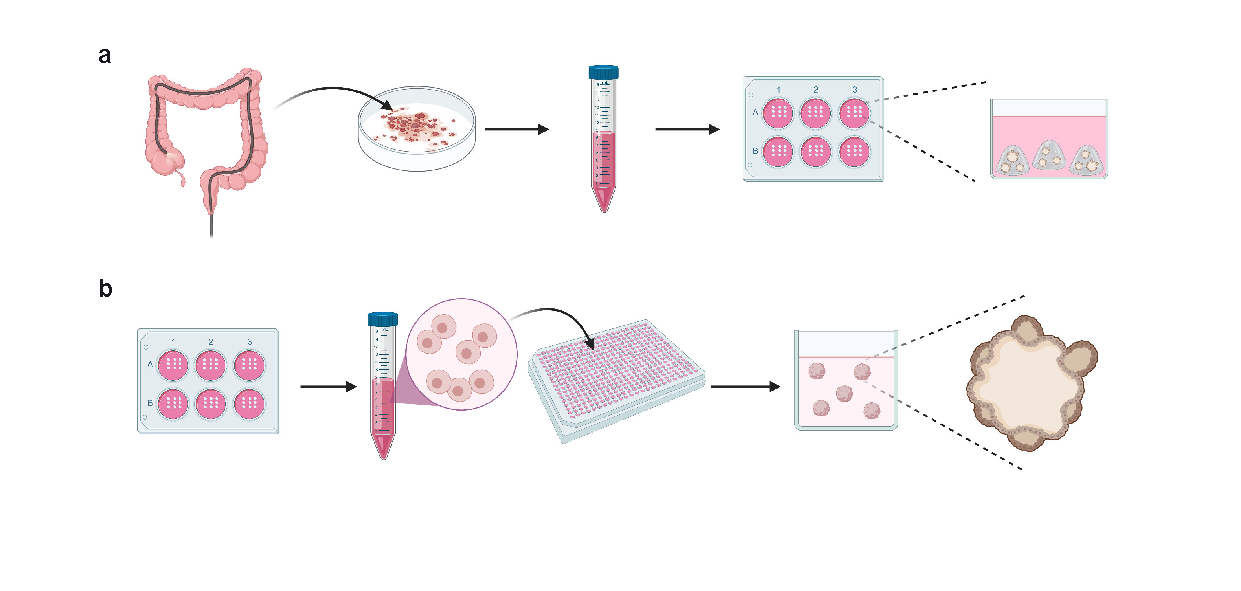
\includegraphics[width=\textwidth,
                height=\textheight,
                keepaspectratio]{figures/promise/pdf/fig_0_1.pdf}
\caption[Core organoid liquid handling methods]{\textbf{Core organoid liquid handling methods a} Organoid isolation procedure. Colorectal cancer tissue biopsies were collected via endoscopy, enzymatically removed from extracellular matrix proteins, washed and resuspended in basal membrane extract hydrogel. After solidification of hydrogel domes, organoids were overlayed with growth factor rich culture medium. \textbf{b} Organoid high-throughput experimentation. Colorectal cancer organoids were harvested, partially digested, seeded in hydrogel-coated 384-well plates. Figure produced with Biorender}
\label{fig_110}
\end{figure}

\subsection{Mouse Organoid seeding during compound testing}
Mouse organoid screening was performed as described above with slight modifications. Clotting of organoid fragments was avoided by adding 10 U/ml of bovine DNAse1 to the medium during filtration. The cell viability of digested fragment suspensions was estimated using Cell-Titer-Glo (Promega). 40μl of cell suspension was mixed with 40μl of undiluted reagent and measured after 30 minutes on a Mithras plate reader (Berthold). Cell fragments with a viability corresponding to 5000 units were seeded per well on pre-coated 384 well microclear assay plates (Greiner) using a Multidrop peristaltic pump robot (Thermo Fischer Scientific) analogous to the human organoid seeding protocol outlined above. 

\subsection{Compound Libraries and Treatment for Patient derived Organoids}
Two compound libraries were used for profiling: A library containing 63 clinically relevant drugs (clinical cancer library) and a large library of 464 compounds targeting kinases and stem cell or developmental pathways associated genes (KiStem library). The clinical cancer library was manually curated by relevance for current (colorectal) cancer therapy, mechanism of action and potential clinical applicability. Compounds of this library are in clinical use or at least in phase I/II clinical trials. Five concentrations per compound were screened (five-fold dilutions). The concentrations were determined by analysis of literature data from previous 3D and 2D drug screens and own experiments. The KiStem library includes 464 compounds targeting a diverse set of kinases and stem cell relevant pathways. All compounds in this library were used in a concentration of 7.5μM. All compounds were obtained from Selleck chemicals. Compounds of both libraries were arranged in an optimized random layout. Compound libraries were stored in DMSO at -80 C.
\bigbreak
After 72 hours of expansion at 37C, medium was aspirated from all organoid screening plates and replaced with fresh ENA medium devoid of Y-27632, resulting in 45μl volume per well. Drug libraries were diluted in basal medium and subsequently 5μl of each compound was distributed to screening plates. 
All liquid handling steps were performed using a Biomek FX robotic system (Beckmann Coulter). Plates were sealed and incubated with the compounds for four days. All PDO lines underwent profiling with the clinical cancer library, while the KiStem library was used with 13 PDO lines.

\begin{figure}[h]
\centering
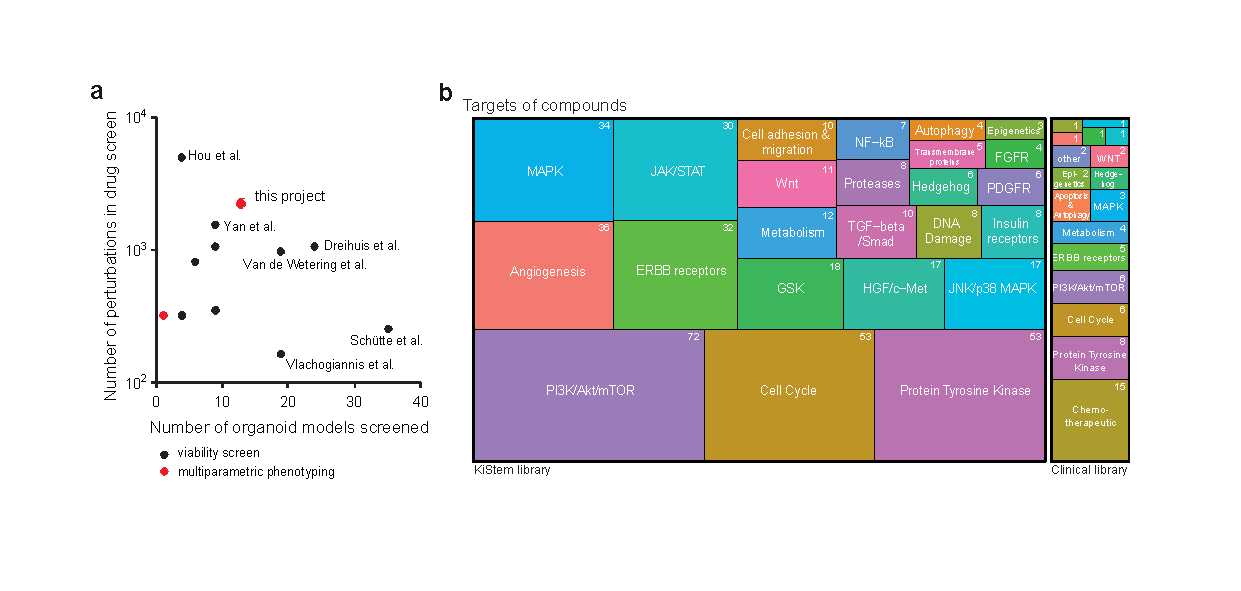
\includegraphics[width=\textwidth,
                height=\textheight,
                keepaspectratio]{figures/promise/pdf/fig_1_3.pdf}
\caption[Dataset dimensions and compound library overview]{\textbf{Dataset dimensions and compound library overview a} Number of organoid models and number of perturbations in previous publications reporting high-throughput drug screenings with patient derived cancer organoids, \textbf{b} Graphical representation of the compound libraries used for drug screening in this project: A library targeting kinases and stem cell pathways (KiStem library, 464 compounds) and a clinical library with 63 drugs in 5 concentrations. Figure created with support from Johannes Betge and adapted from \textit{The drug-induced phenotypic landscape of colorectal cancer organoids} \parencite{betgeDruginducedPhenotypicLandscape2022}}
\label{fig_137}
\end{figure}

\subsection{Compound Libraries and Treatment for Mouse Organoids}
Two compound libraries were used for profiling: The KiStem library (see above) as well as a library of FDA-approved small molecules. For both the KiStem library and the FDA-approved library, one single concentration was used. All compounds in this library were used in a concentration of 7.5μM. All compounds were obtained from Selleck chemicals. Compounds of both libraries were arranged in an optimized random layout and complete compound libraries were stored in DMSO at -80 C.
\bigbreak
Mouse Organoids were treated similar to Patient derived Organoids with slight modifications: After 72 hours of organoid expansion in WENRAS, the medium was changed to ENR and compound libraries were added using a BiomekFX (Beckmann Coulter). All Mouse Organoids were profiled with the KiStem library and FDA-approved compound library.

\subsection{Automated Microscopy}
After 96h of small molecule treatment, Image-IT DeadGreen (Thermo Fisher) was added to the cultures with a Multidrop dispenser (Thermo Fisher) in 100nM final concentration and incubated for four hours. Afterwards, medium was removed and organoid cultures were fixed with 3\% PFA in PBS with 1\% BSA. Fixed plates were stored at 4° C for up to three days before permeabilization and staining. On the day of imaging, organoids were permeabilized with 0.3\% Triton-X-100 and 0.05\% Tween in PBS with 1\% BSA and stained with 0.1μg/ml TRITC-Phalloidin (Sigma) and 2μg/ml DAPI (Sigma). All liquid handling steps were performed with a BiomekFX. Screening plates were imaged with an Incell Analyzer 6000 (GE Healthcare) line-scanning confocal fluorescent microscope. We acquired 4 fields per well with z-stacks of 16 slices at 10x magnification. The z-steps between the 16 slices had a distance of 5μm, the depth of field of each slice was 3.9μm.

\subsection{Luminescence Viability Read Out of Patient Derived Organoids}
Organoid screening plates undergoing ATP-based viability testing were cultured in solid, white plates (Greiner) treated with 30μl CellTiter-Glo reagent after medium aspiration with a Biomek FX. After incubation for 30 minutes, luminescence levels were measured with a Mithras reader (Berthold technologies).

Raw luminescence data of each plate were first normalized using the Loess-fit method in order to correct for edge effects where increased luminescence intensity was observed along the edges of each plate. Subsequently, each plate was normalized by division with the median luminescence intensity of the DMSO controls. Drug response Hill curves (DRC) were fitted and area under the curve values were calculated for each DRC using the ‘PharmacoGx’ \parencite{smirnovPharmacoGxPackageAnalysis2016} R/Bioconductor package.

\subsection{Luminescence Viability Read Out of Patient Derived Organoids of Mouse Organoids}
For selected compounds, before compound addition, organoid viability was measured using Cell-Titer-Glo (Promega). Cell viability was measured after compound exposure as described above. The pre-treatment viability of organoids was used to estimate growth-rate controlled dose-response curves according to \parencite{hafnerGrowthRateInhibition2016} Measurements of GR metrics for were not robust for slow proliferating WT lines. Therefore, these lines were omitted in the analysis.

\section{Image analysis}

\subsection{Image Processing}
Microscopic image z-stacks were compressed to HDF5 format for archival and underwent maximum contrast projection using the R/Bioconductor package MaxContrastProjection developed by Jan Sauer for further processing of the images. Standard image features, including shape, moment, intensity, and Haralick texture features on multiple scales, were extracted using the R/Bioconductor package EBImage \parencite{pauEBImagePackageImage2010}. Of note, the strong diversity of unperturbed organoid phenotypes between organoid lines did not allow the definition of a core set of individual reproducible descriptive features across all screened organoids. Therefore, no correlation-based filtering of features was done, allowing comparisons between different lines. Out-of-focus objects were manually and programmatically removed from the dataset using a custom classifier developed by Jan Sauer.

\begin{figure}[h]
\centering
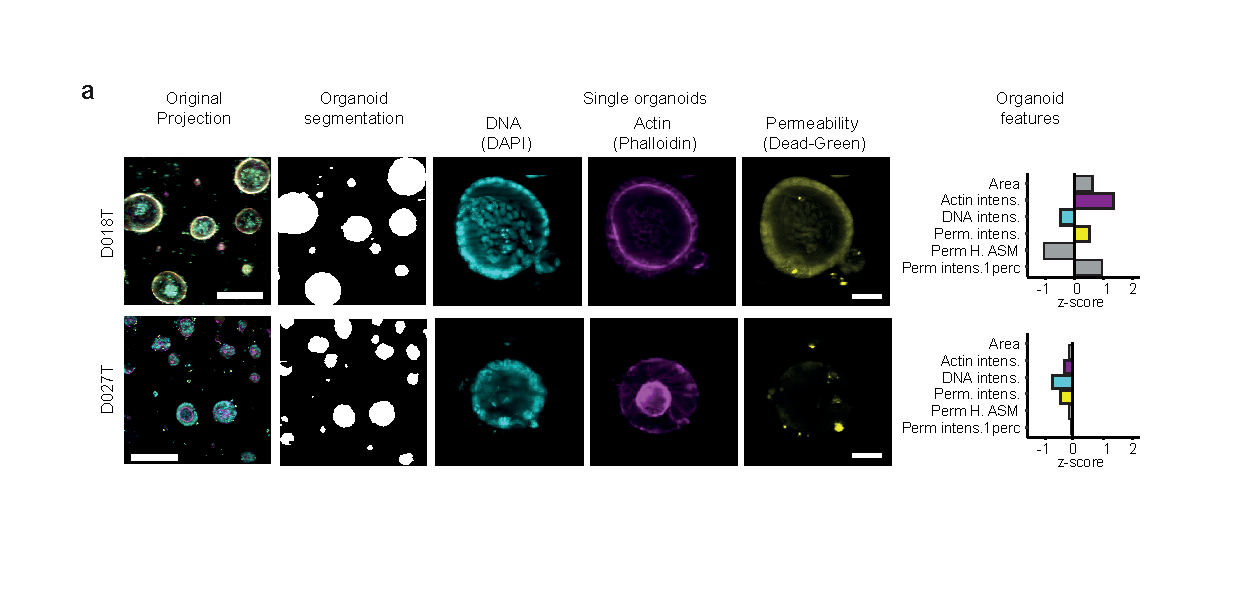
\includegraphics[width=\textwidth,
                height=\textheight,
                keepaspectratio]{figures/promise/pdf/fig_1_2.pdf}
\caption[Image-based profiling method overview]{\textbf{Image-based profiling method overview a} The image-processing pipeline illustrated with representative example images from two organoid lines: Organoids were imaged at multiple layers along the z-axis. Images were projected using a maximum contrast projection and segmented using a convolutional neural network, both designed and implemented by Jan Sauer. Descriptive features were extracted from all three channels to quantify phenotypes. Feature plots show the median phenotype of unperturbed organoids, six example features (Area, Phalloidin intensity, DAPI intensity, FITC intensity, FITC Haralic angular second moment (ASM) and FITC intensity 1-percentile) and their z-scores relative to all profiled organoid lines are shown. Figure created with support from Jan Sauer (data processing) and Johannes Betge (graphical presentation). Figure adapted from \textit{The drug-induced phenotypic landscape of colorectal cancer organoids} \parencite{betgeDruginducedPhenotypicLandscape2022}}
\label{fig_135}
\end{figure}

\subsection{Feature Processing and Treatment-Induced Phenotypes}
The dimensionality of calculated single-organoid morphological features was reduced using a principal component analysis (PCA) that was performed on the entire datasets (patient derived and mouse organoids separately) to reduce the dimensionality. 25 principal components were selected, explaining ca. 80\% of the total variance within both datasets. These 25 principal components were used for further analysis of single-organoid morphology and were averaged on a per-well level for the MOFA analysis.
\bigbreak
For treatment activity estimation, a logistic regression classifier was trained per line and treatment (and per concentration where applicable) to differentiate individual treated organoids from negative controls based on the PCA-transformed features. Drugs were categorized as either active or inactive based on the accuracy of the model. The direction of the decision plane's normal vector was used as the treatment effect vector. Drugs were clustered based on the cosine similarity of their normal vectors.


\section{Multi-omics factor analysis}
\subsection{Model training of Patient Derived Organoids}
A multi-omics factor analysis model \parencite{argelaguetMultiOmicsFactorAnalysis2018b} was trained based on a set of five modalities describing unperturbed organoid lines:

\begin{itemize}
    \item organoid size estimated based on log-normal model fit of all DMSO treated organoids [22 replicates, 1 feature]
    \item organoid somatic mutations as determined by amplicon sequencing [20 replicates, 12 features]
    \item organoid transcript expression of the top 10\% genes with the highest coefficient of variance after robust multi-array average normalization [22 replicates, 3222 features]
    \item organoid morphology as determined by averaging DMSO treated morphological profiles [22 replicates, 25 features]
    \item organoid drug activity as determined by AUROC score of logistic regression models for drugs that were defined as active in at least one observation [22 replicates, 252 features]
\end{itemize}


Input data was scaled and the MOFA model was trained with default MOFA2 training parameters and a number of 3 factors. The number of factors was chosen given the limited number of observations in the training data. The further analysis focused on the first two factors, which correlated with prominent visible organoid phenotypes. Gene set enrichment analysis and Reactome pathway enrichment of factor loadings was performed using the clusterprofiler R package \parencite{yuClusterProfilerPackageComparing2012}. Enrichment of drug targets within factor loadings was tested using ANOVA by fitting a linear model, \textit{lm(factor loading vs. target)}. Drug targets that were represented with at least three small molecule inhibitors were included in this analysis. The analysis was run using the MOFA docker container available from https://hub.docker.com/r/gtca/mofa2.

\subsection{Model training of Mouse Organoids}
A multi-omics factor analysis model with k=4 factors was trained and results were analysed as above, with a different set of input data: 
\begin{itemize}
    \item organoid size all DMSO treated organoids (one replicate of Apc-/- organoids was removed from the analysis) [7 replicates, 1 feature]
    \item organoid transcript expression including the top 10\% genes with the highest coefficient of variance after robust multi-array average normalization [8 replicates, 2727 features]
    \item organoid protein expression [12 replicates, 3906 features]
    \item organoid lipid abundance [12 replicates, 397 features]
    \item organoid genotype for the $Apc$ and KrasG12 allele [12 replicates, 2 features]
    \item organoid morphology as determined by averaging DMSO treated morphological profiles (one replicate of Apc\textsuperscript{-/-} organoids was removed from the analysis) [7 replicates, 25 features]
    \item organoid drug activity as determined by AUROC score of logistic regression models for drugs [7 replicates, 1699 features]
\end{itemize}


\subsection{Model projection}
To estimate the factor scores for treatment-induced organoid morphologies, the morphology feature matrix was multiplied with the pseudoinverse of the previously learnt model's factor weight matrix for the organoid morphology modality. 

\smallbreak
The resulting projected factor score matrix was used to estimate the drug-induced biological changes in both patient derived and mouse organoids. Associations between drug targets and projected factor scores of drug treated organoids were identified via ANOVA by fitting a linear model, \textit{lm(projected factor score vs. target)}. For mouse organoids, the model was extended to account for line-wise effects in the modeling, \textit{lm(projected factor score vs. target + organoid-line)}. Drug targets that were represented with at least three small molecule inhibitors were included in the analysis, except in the modeling of individual small molecule effects on mouse organoids.


\section{Biochemical assays}

\subsection{Amplicon Sequencing of Mouse Organoids}
Amplicon sequencing was performed to validate the CRISPR perturbation of \textit{Apc}. DNA from \textit{Apc} targeted and untargeted organoid lines was prepared using the DNA Blood and Tissue Kit (Qiagen), according to the manufacturer’s tissue protocol including an RNAse digestion. The targeted region was PCR amplified using primers F1 and R1. Libraries were sequenced on a MySeq (Illumina) using 100bp single end reads. 

\begin{table}[htb]
\caption{List of Genomic PCR Primers for Amplicon Sequencing}
\label{tab:oligonucleotides} % Label for referencing
\begin{tabularx}{\textwidth}{XlX}
\toprule
\textbf{Reagent or Resource} & \textbf{Sequence} & \textbf{Source} \\
\midrule
Primer F1 & TCCCTACACGACGCTCTTCCGATCTGGAATGTCAGAAGGGAGACC & GATC Biotech \\
%Primer F2 & TCCCTACACGACGCTCTTCCGATCTGAGGAATGTCAGAAGGGAGA & GATC Biotech \\
Primer R1 & AGTTCAGACGTGTGCTCTTCCGATCTCCAACCAGAAATGCCAGTG & GATC Biotech \\
%Primer R2 & AGTTCAGACGTGTGCTCTTCCGATCTGCCAACCAGAAATGCCAGT & GATC Biotech \\
\bottomrule
\end{tabularx}
\end{table}

\subsection{Genomic PCR of the KRAS G12D allele in Mouse Organoids}
To confirm activation of oncogenic $Kras$ in 4-Hydroxytamoxifen treated lines, genomic DNA was isolated from all 4 organoid lines as described above. Presence or absence of the Lox-STOP-Lox cassette was evaluated by PCR according to the $Kras^{G12D/+}$ conditional PCR protocol by Tyler Jacks’ group \parencite{jacksonAnalysisLungTumor2001}. Briefly, primers \#2 and \#3 were used for genotyping on genomic DNA using the Q5 PCR protocol (NEB).

\begin{table}[htb]
\caption{List of Primers for validating KRAS conditional PCR}
\label{tab:kras} % Label for referencing
\begin{tabularx}{\textwidth}{XlX}
\toprule
\textbf{Reagent or Resource} & \textbf{Sequence} & \textbf{Source} \\
\midrule
Primer \#2 & CTCTTGCCTACGCCACCAGCT & GATC Biotech \\
Primer \#3 & AGCTAGCCACCATGGCTTGAGTAAGTCTGCA & GATC Biotech \\
\bottomrule
\end{tabularx}
\end{table}

\subsection{Western Blot of Patient derived Organoids}
Organoids seeded in 6-well plates were cultured in Matrigel (Corning). After 3-days incubation with WYE-132, organoids were collected, and cells were isolated using Matrisperse (Corning) for 40 minutes on a rocking table. Cells were subsequently lysed in RIPA buffer (Thermo Fisher Scientific) supplemented with Protease inhibitors (Complete Mini, Roche) and Phosphatase inhibitors 1 and 2 (Sigma), followed by sonication (Branson Sonifier, Heinemann). Protein concentrations of supernatants were measured using the Pierce BCA kit (Thermo Fisher Scientific) according to the manufacturers protocol. Lysates were mixed with an SDS-loading buffer and heated to 99 C for 5 minutes. Proteins were separated by SDS–PAGE in MOPS running buffer and transferred to a nitrocellulose membrane. Membranes were blocked with 5\% (w/v) skim milk in PBS containing 0.1\% (v/v) Triton X-100 (PBS-T). Western Blotting was performed with following antibodies (all in 5\% (w/v) skim milk, PBS-T): anti-IRS1 (1:1000, 06-248, Sigma–Aldrich), anti-HSP-90 (1:1000, sc-13119, Santa Cruz), anti-Mouse-IgG-HRP (1:10000, Sigma–Aldrich). ECL Western Blotting W1001 (Promega) was used for visualization of bands.

\begin{table}[htb]
\caption{List of Antibodies used in experiments}
\label{tab:antibodies} % Label for referencing
\begin{tabularx}{\textwidth}{Xll}
\toprule
\textbf{Reagent or Resource} & \textbf{Source} & \textbf{Identifier} \\
\midrule
Anti-IRS1 (rabbit) & Sigma–Aldrich & 06-248 \\
Anti HSP-90 (mouse) & Santa Cruz & 13119 \\
Anti-ERK (p44/42 MAPK) (rabbit) & Cell Signaling & 4695 \\
Anti-phospho-ERK (phospho-p44/42 MAPK) (rabbit) & Cell Signaling & 4370 \\
Anti-beta-actin HRP (mouse) &  &  \\
\bottomrule
\end{tabularx}
\end{table}

\subsection{Western Blot of Mouse Organoids}
Organoids were cultured in Matrigel (Corning). Organoids were collected, and cells were isolated using Matrisperse (Corning) for 40 minutes on a rocking table. Isolated organoids were lysed in RIPA buffer (Sigma) with Protease inhibitor (Sigma) and Phosphatase inhibitor 3 (Sigma). Protein concentration was measured using the Pierce BCA kit (Thermo Fischer Scientific) according to the manufacturers protocol. Lysates were mixed with an SDS-loading buffer and heated to 99 C for 5 minutes. Samples were loaded onto NuPage gels (Thermo Fischer Scientific), separated in MOPS running buffer and transferred to a nitrocellulose membrane. Membranes were blocked with 5\% (w/v) skim milk in PBS containing 0.1\% (v/v) Triton X-100 (PBS-T). Western Blotting was performed with following antibodies (all in 5\% (w/v) skim milk, PBS-T): anti-p(hospho)-Erk (1:2000, Cell Signaling, ID 4370), anti-Erk (1:1000, Cell Signaling, ID 4695) and anti-beta-actin-HRP secondary antibody (1:150,000).

\subsection{Mouse Organoid Growth Patterns}
Organoids were passaged and seeded in 4 different growth media with medium changes every 48h. Images were taken 120h after seeding with 4x magnification on a Zeis Axiovert. 

\subsection{RT-qPCR of Patient derived Organoids}
Organoids seeding and treatment timing was performed in accordance with the image-based profiling protocol. After 120h of growth, total RNA was isolated using the RNAEasy Mini kit (Qiagen) without additives. cDNA synthesis was done with Verso cDNA kit (Thermo Fisher Scientific), and RT-qPCR was performed using the SYBR Green Mix (Roche) on a LightCycler480 system (Roche). UBC expression levels were used as controls.

\begin{table}[htb]
\caption{List of RT-qPCR Primers}
\label{tab:qpcr} % Label for referencing
\begin{tabularx}{\textwidth}{lXll}
\toprule
\textbf{Reagent or Resource} & \textbf{Organism} & \textbf{Sequence} & \textbf{Source} \\
\midrule
LGR5 F & Human & TTCCCAGGGAGTGGATTCTAT & GATC Biotech \\
LGR5 F & Human & ACCAGACTATGCCTTTGGAAAC & GATC Biotech \\
UBC F & Human & CTGATCAGCAGAGGTTGATCTTT & GATC Biotech \\
UBC R & Human & TCTGGATGTTGTAGTCAGACAGG & GATC Biotech \\
Axin2 F & Mouse & GAGAGTGAGCGGCAGAGC & GATC Biotech \\
Axin2 R & Mouse & CGGCTGACTCGTTCTCCT & GATC Biotech \\
Ccnd F & Mouse & TTTCTTTCCAGAGTCATCAAGTGT & GATC Biotech \\
Ccnd R & Mouse & TGACTCCAGAAGGGCTTCAA & GATC Biotech \\
Sdha F & Mouse & TGTTCAGTTCCACCCCACA & GATC Biotech \\
Sdha R & Mouse & TCTCCACGACACCCTTCTGT & GATC Biotech \\
Hprt F & Mouse & CCTCCTCAGACCGCTTTTT & GATC Biotech \\
Hprt R & Mouse & CCTCCTCAGACCGCTTTTT & GATC Biotech \\
\bottomrule
\end{tabularx}
\end{table}

\subsection{RT-qPCR of Mouse Organoids}
Organoids were passaged and seeded in 4 different growth media with medium changes every 48h. After 120h, organoid RNA was isolated using the RNAEasy Kit (Qiagen) with beta-Mercaptoethanol (Invitrogen) and a DNAse digestion step. cDNA was synthesized using Oligo-dT primers (Thermo Fisher Scientific), RiboLock Ribonuclease inhibitor (Thermo Fisher Scientific) and Revert Aid H Minus reverse transcriptase (Thermo Fisher Scientific). RT-qPCR was performed using the ROCHE UPL kit (Roche) on a LightCycler480 system (Roche). Sdha and Hprt expression levels were used as controls and averaged. Relative transcript abundance was measured using the ddCT method.
 
\subsection{Proteomics Profiling of Mouse Organoids}
Organoids were cultured according to the image-based profiling protocol. Samples were isolated with Matrisperse (Corning) as described above. Isolated organoids were lysed in Ammonium Bicarbonate lysis buffer (50mM, pH 8.2) with 2.5\% w/v SDC and 25U/ml Benzonase. 
Samples were handed over to the Proteomics core facility at the German Cancer Research Center. There, a 1D-SDS-PAGE of the lysate was run followed by fractionation. Gel pieces were extracted, cysteins residues reduced by DTT and carbamidomethylated using iodoacetamide. The samples were digested with Trypsin overnight.
Resulting peptides were loaded on a cartridge trap column, packed with Acclaim PepMap300 C18, 5µm, 300Å wide pore (Thermo Fischer Scientific) and segregated in a 60 min gradient from 3\% to 40\% ACN on a nanoEase MZ Peptide analytical column (300Å, 1.7 µm, 75 µm x 200 mm, Waters). Eluted peptides were analyzed by an online coupled Q-Exactive-HF-X mass spectrometer.

\subsection{Lipidomics Profiling of Mouse Organoids}
Organoids were cultured according to the the image-based profiling protocol and prepared for analysis according to the method developed for proteomics profiling (above). 
Isolated organoids were processed by the Lipidomics and Metabolomics core facility. 
After lipid extraction, isolates were analysed using a Qtrap 6500 Mass Spectrometer (SCIEX) coupled to a NanoMate (NanoMate) electrospray source. Metabolome profiles were generated and handed over to the authors for downstream imputation and analysis.

\subsection{Transcript Expression Profiling of Patient derived Organoids}
Organoid RNA was isolated from 19 patient derived organoid lines with the RNeasy mini kit after snap freezing organoids on dry ice. Samples were hybridized on Affymetrix U133 plus 2.0 arrays. Raw microarray data were normalized using the robust multi-array average (RMA) method \parencite{irizarryExplorationNormalizationSummaries2003} followed by quantile normalization as implemented in the ‘affy’ \parencite{gautierAffyAnalysisAffymetrix2004} R/Bioconductor \parencite{huberOrchestratingHighthroughputGenomic2015} package. Differential gene expression analyses were performed using a moderated t-test as implemented in the R/Bioconductor package ‘limma’ \parencite{ritchieLimmaPowersDifferential2015}. Gene set enrichment analyses were performed using ConsensusPathDB \parencite{kamburovConsensusPathDBMoreComplete2011} for discrete gene sets or GSEA as implemented in the ‘fgsea’ R/Bioconductor package for ranked gene lists.

\subsection{Transcript Expression Profiling of Mouse Organoids}
Mouse organoids were cultured according to the image-based profiling protocol. Briefly, organoid models were seeded and cultured for 72h in WENRAS and additional 96h in ENR. Samples were harvested after 7 days and RNA was isolated using the RNAEasy Kit (Qiagen) as described above. Transcript expression levels were measured using MoGene-2\_0-st chips (Affymetrix).
Differential gene expression analyses were performed analogous to Patient derived Organoids.

\end{flushleft}